\documentclass[10pt,openany]{article}
\usepackage{ctex} 
\usepackage{geometry,graphicx,xcolor,color}
\geometry{
	a4paper,
	top=25.4mm, bottom=25.4mm,
	left=20mm, right=20mm,
	headheight=2.17cm,
	headsep=4mm,
	footskip=12mm
}
\usepackage[all,pdf]{xy}
\usepackage{amssymb,amsmath,mathrsfs}             
\usepackage{mathpazo}
\usepackage[nofontspec]{newpxtext}
\usepackage{array}
\usepackage{amsmath}
\usepackage{amssymb}
\usepackage{enumerate}
\usepackage{amsthm}
\usepackage{bm}
\usepackage{mathtools}
\usepackage{mathrsfs}
\usepackage{tcolorbox}
\usepackage{indentfirst}
\usepackage{setspace}
\usepackage{subfigure} 
\usepackage{tkz-fct}
\usetikzlibrary{calc,intersections,through,backgrounds,3d}
\usepackage{tkz-euclide}
\usepackage{pgfplots}
\usepackage{booktabs}
\usepackage{float}
\usepackage[graphicx]{realboxes}
\usepackage{fancyhdr}

\definecolor{winered}{rgb}{0.5,0,0}
\definecolor{structurecolor}{RGB}{122,122,142}
\definecolor{main}{HTML}{3D445F}
\definecolor{second}{HTML}{627581}
\definecolor{third}{HTML}{333333}
\definecolor{deepgreen}{HTML}{2F5E4E}  
\definecolor{purple}{HTML}{512E5F}   

\usepackage{hyperref}
\hypersetup{colorlinks = true, linktoc=all, linkcolor=blue, urlcolor=winered}


\usepackage{amsthm}
% 设定颜色(假设你在别处定义了 \color{main} 等)
\usepackage{xcolor}
\usepackage{etoolbox}
% 定义定理风格
\usepackage{amsthm}
\newtheoremstyle{defstyle}
{0.3cm}{0.3cm}{\fangsong}{-1cm}{\bfseries\color{main}}{}{0.5em}
{\indent 【\thmname{#1} \thmnumber{#2}】\ifthenelse{\equal{#3}{}}{}{~\thmnote{(#3)}}}

\newtheoremstyle{thmstyle}
{0.3cm}{0.3cm}{\kaishu}{-1cm}{\bfseries\color{second}}{}{0.5em}
{\indent 【\thmname{#1} \thmnumber{#2}】\ifthenelse{\equal{#3}{}}{}{~\thmnote{(#3)}}}

\newtheoremstyle{remstyle}
{0.3cm}{0.3cm}{\kaishu}{-1cm}{\bfseries\color{third}}{}{0.5em}
{\indent 【\thmname{#1} \thmnumber{#2}】\ifthenelse{\equal{#3}{}}{}{~\thmnote{(#3)}}}

\newtheoremstyle{exastyle}
{0.3cm}{0.3cm}{\kaishu}{-1cm}{\bfseries\color{deepgreen}}{}{0.5em}
{\indent 【\thmname{#1} \thmnumber{#2}】\ifthenelse{\equal{#3}{}}{}{~\thmnote{(#3)}}}

\newtheoremstyle{prostyle}
{0.3cm}{0.3cm}{\kaishu}{-1cm}{\bfseries\color{purple}}{}{0.5em}
{\indent 【\thmname{#1} \thmnumber{#2}】\ifthenelse{\equal{#3}{}}{}{~\thmnote{(#3)}}}

\theoremstyle{thmstyle} %theorem style
\newtheorem{theorem}{定理}[subsection]
\theoremstyle{defstyle} % definition style
\newtheorem{definition}[theorem]{定义}
\newtheorem{lemma}[theorem]{引理}
\newtheorem{corollary}[theorem]{推论}
\theoremstyle{prostyle} % proposition style
\newtheorem{proposition}[theorem]{命题}
\newtheorem{property}[theorem]{性质}
\theoremstyle{exastyle} 
\newtheorem{example}[theorem]{例}
\AtEndEnvironment{example}{\hfill \( \diamondsuit \)}
\theoremstyle{remstyle} 
\newtheorem{remark}[theorem]{注}

\renewenvironment{proof}[1][证明]{\par\underline{\textbf{#1.}} \;\fangsong}{\qed\par}
\newenvironment{solution}{\par\underline{\textbf{解.}} \;\fangsong}{\qed\par}
\newcommand{\intro}[1]{\rightline{\parbox[t]{5cm}{\footnotesize \fangsong\quad\quad #1 }}}

\AtEndEnvironment{proof}{\vspace{1.5ex}}
\AtEndEnvironment{solution}{\vspace{1.5ex}}

\usepackage{titlesec, titletoc}
\linespread{1.2} 				
\usepackage{fancyhdr}
\fancyhf{}
\renewcommand{\headrule}{\color{structurecolor}\hrule width\textwidth}
\pagestyle{fancy}
\renewcommand{\headrulewidth}{1pt}
\fancypagestyle{plain}{\renewcommand{\headrulewidth}{0pt}\fancyhf{}\renewcommand{\headrule}{}}

\fancyhead[c]{\color{structurecolor}\kaishu\rightmark}
\fancyfoot[c]{\color{structurecolor}\small\thepage}


\titleformat{\section}[frame]{\normalfont\color{structurecolor}}{\footnotesize \enspace \large \textcolor{structurecolor}{\S \,\thesection}\enspace}{6pt}{\Large\filcenter \bf \kaishu }


\titleformat{\subsection}[hang]{\bfseries}{\large\bfseries\color{structurecolor}\thesubsection\enspace}{1pt}{\color{structurecolor}\large\bfseries\filright}

\titleformat{\subsubsection}[hang]{\bfseries}{\large\bfseries\color{structurecolor}\thesubsubsection\enspace}{1pt}{\color{structurecolor}\large\bfseries\filright}

\usepackage{titling}
\renewcommand*{\maketitle}{
	\begin{titlepage}
		\newgeometry{margin = 0in}
		\parindent=0pt
		\includegraphics[width=\linewidth]{cover.png}
		\vfill
		\begin{center}
			\parbox{0.618\textwidth}{
				\hfill {\bfseries \Huge \thetitle} \\[0.6pt]  
				\rule{0.618\textwidth}{4pt} \\ 
			}
		\end{center}
		\vfill
		\begin{center}
			\parbox{0.618\textwidth}{
				\hfill\Large
				\kaishu 
				\begin{tabular}{r|}
					\textbf{2025 Summer} \\
					作者:\theauthor \\ 
					时间:\thedate \\
				\end{tabular}
			}
		\end{center}
		\vfill
		\begin{center}
			\parbox[t]{0.7\textwidth}{\centering \kaishu}
		\end{center}
		\vfill
	\end{titlepage}
	\restoregeometry
	\thispagestyle{empty}
}

\newcommand{\T}{^{\text{T}}}
\newcommand{\Her}{^{\text{H}}}
\newcommand{\F}{\mathbb{F}}
\newcommand{\gf}{\text{GL}_n(\mathbb{F})}
\newcommand{\C}{\mathbb{C}}
\newcommand{\R}{\mathbb{R}}
\newcommand{\Q}{\mathbb{Q}}
\newcommand{\n}{^{n \times n}}
\newcommand{\mn}{^{m \times n}}
\newcommand{\nm}{^{n \times m}}
\newcommand{\tz}{\mathrm{char} \;}
\newcommand{\tr}{\mathrm{tr}}
\newcommand{\diag}{\mathrm{diag}}
\newcommand{\oneb}{\underline{\hspace{1em}}\hspace{0.001em}}
\newcommand{\twob}{\oneb\oneb}
\newcommand{\fourb}{\twob\twob}
\newcommand{\tenb}{\twob\twob\twob\twob\twob}
\newcommand{\tideparallel}{%  
	\mathrel{%  
		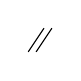
\begin{tikzpicture}[scale=0.2, baseline={([yshift=-0.5ex]current bounding box.center)}]  
			\draw[thin] (0,0) -- (1,1.5);  
			\draw[thin] (0.5,0) -- (1.5,1.5);  
		\end{tikzpicture}%  
	}%  
}  
\newcommand{\fourch}[4]
{\\[3pt]
	\begin{tabular}
		{*{4}{@{}p{4cm}}}
		A.~#1 & B.~#2 & C.~#3 & D.~#4
	\end{tabular}	
}
\newcommand{\fourchh}[4]
{\\[5pt]
	\begin{tabular}
		{*{4}{@{}p{20cm}}}
		A.~#1 \\[5pt] B.~#2 \\[5pt] C.~#3 \\[5pt] D.~#4
	\end{tabular}	
}
\newcommand{\fourchhh}[4]
{\\[3pt]
	\begin{tabular}
		{*{4}{@{}p{7.5cm}}}
		A.~#1 & B.~#2 \\[2pt] C.~#3 & D.~#4
	\end{tabular}	
}
\newcommand{\independent}{\perp\!\!\!\perp}
\everymath{\displaystyle}
\allowdisplaybreaks




\begin{document}

\pagestyle{fancy}
\lhead{Lecture 2}
\chead{illusion \& FzRainD}
\rhead{\today}

\setcounter{section}{1}
\section{可逆矩阵和行列式}

进入 \S 2 节,我们本节的任务主要是延续上节的讨论,探寻对方阵而言,什么样的方阵能在 \( \F\n \) 中可逆. 进一步,如果 \( A \) 可逆,那么解线性方程组 \( AX=\beta \) 就变得非常容易了,只需要 \( X=A^{-1}AX=A^{-1}\beta \). 我们离这种 \( n \) 个方程组成的关于 \( n \) 个变元的线性方程组的公式解,只有一步之遥,那就是如何给出 \( A^{-1} \) 的表达式?
但这些假设的前提是,我们已经知道矩阵 \( A \) 可逆,当务之急应该是找出一个判定 \( A \) 可逆的法则. 

\subsection{可逆矩阵和一般线性群}
\begin{definition}[可逆矩阵]
	设 \( A \in \F\n \),称 \( A \) 是可逆矩阵,若存在 \( B \in \F\n \) 使得 \( AB=BA=E_n \). 此时,一般记 \( B=A^{-1} \). 从定义可见,可逆矩阵与矩阵本身互为逆矩阵,即 \( A^{-1} \) 的逆矩阵也为 \( A \).
	\label{2.1.1}
\end{definition}

\begin{property}[可逆矩阵的性质]
	若矩阵 \( A, B \in \F\n \) 可逆,那么
	\begin{enumerate}[(1)]
		\item 矩阵 \( A \) 的逆元 \( B=A^{-1} \) 必定唯一;
		\item (穿脱法则 I) \ 矩阵 \( AB \) 也可逆,其逆元 \( (AB)^{-1}=B^{-1}A^{-1} \);
		\item (穿脱法则 II) \ 对一列方阵 \( \{A_k\}_{1 \leq k \leq n} \) 为可逆矩阵,那么 \( A_1A_2\cdots A_n \) 也可逆,且 \( (A_1A_2\cdots A_n)^{-1}=A_n^{-1}A_{n-1}^{-1}\cdots A_1^{-1} \);
		\item (转置与取逆的协调) \ \( A\T \) 也可逆,且 \( (A\T)^{-1}=(A^{-1})\T \).
	\end{enumerate}
	\label{2.1.2}
\end{property}

\begin{proof}
	(1) 设还有 \( C \in \F\n \) 使得 \( AC=CA=E_n \). 那么 \( C=E_nC=(BA)C=B(AC)=BE_n=B \). (2) 只需要验证定义,\( (B^{-1}A^{-1})(AB)=B^{-1}(A^{-1}A)B=B^{-1}E_nB=B^{-1}B=E_n \). 另一方面,\( (AB)(B^{-1}A^{-1})=E_n \) 是类似的. (3) 完全等同 (2),只需要用归纳法. (4) 验证 \( (A^{-1})\T(A\T)=(AA^{-1})\T=E_n\T=E_n \). 同理 \( (A\T)(A^{-1})\T= E_n \).
\end{proof}

\begin{example}[初等矩阵]
	初等矩阵均可逆. 且它们的逆矩阵十分容易求出. 可以自行验证如下的结论:
	\[ E(i,j(c))^{-1}=E(i,j(-c)), \; E(i(c))^{-1}=E(i(c^{-1})) \ (c \neq 0), \; E(i,j)^{-1}=E(i,j). \]
	现在我们明白了,所谓初等矩阵对应操作的逆操作,无非就是左乘初等矩阵的逆矩阵.
	\label{2.1.3}
\end{example}

\begin{example}[单位矩阵]
	单位矩阵显然可逆,且 \( E_n^{-1}=E_n \).
\end{example}

\begin{example}
	若矩阵 \( A,B \) 可逆,那么 \( A+B \) 不一定可逆,例如取 \( A=E_n, \; B=-E_n \),那么 \( A+B=O \). 而必定不存在矩阵 \( C \in \F\n \) 使得 \( CO=OC=E_n \)!
	\label{2.1.5}
\end{example}

事实上,在性质 \ref{2.1.2} 的证明中我们只用到了矩阵乘法的结合律,矩阵乘法存在幺元,以及可逆矩阵的定义,即定义 \ref{2.1.1}. 这提示我们性质 \ref{2.1.2} 应该具有一般性. 接下来,我们将矩阵环 \( \F\n \) 的乘法部分作如下提炼,就得到群的定义.

\begin{definition}[群]
	设 \( G \) 是一个非空集合,其上存在一个二元运算 \( \cdot: G \times G \to G \),满足
	\begin{enumerate}
		\item[(1)] \textbf{结合律} \( (ab)c=a(bc) \);
	\end{enumerate}
	那么称 \( (G,\cdot) \) 为一个半群,进一步,如果还有
	\begin{enumerate}
		\item[(2)] \textbf{幺元性质} 存在 \( e \in G \) 使得 \( ae=ea=a \);
	\end{enumerate}
	那么称 \( (G,\cdot) \) 为一个幺半群. 进一步,如果还有
	\begin{enumerate}
		\item[(3)] \textbf{存在逆元} 对 \( a \in G \),存在 \( a^{-1} \in G \) 使得 \( a(a^{-1})=(a^{-1})a=e \);
	\end{enumerate}
	\textbf{那么称 \( (G,\cdot) \) 为一个群. } 进一步,如果还有
	\begin{enumerate}
		\item[(4)] \textbf{交换律} \( ab=ba \).
	\end{enumerate}
	那么称 \( (G,\cdot) \) 为一个交换群或者 Abel 群. 上述定义中,\( a,b,c \in G \) 都是任取的.
\end{definition}

上述定义我们一点都不陌生,我们可以很清楚地发现,环和域的定义几乎完全就是满足上述定义的两种运算的拼接,并额外满足两种运算的协调性而已. 轻而易举地获得下面的例子.

\begin{example}
	设 \( \F \) 是域,那么 \( (\F,+) \) 在数的通常加法下为一个 Abel 群,记 \( \F^*:=\F \textbackslash \{0\} \),那么 \( (\F,\cdot) \) 在数的通常乘法下为一个 Abel 群. 
\end{example}

\begin{example}
	设 \( \F\n \) 是域 \( \F \) 上的全矩阵环,那么 \( (\F\n,+) \) 在通常矩阵的加法下为一个 Abel 群. 
\end{example}

\begin{example}
	记 \( \gf:=\{ A \in \F\n \mid \exists \ B \in \F\n, \; AB=BA=E_n \} \),也就是 \( \F\n \) 中的可逆矩阵全体. 那么 \( (\gf,\cdot) \) 在配备通常矩阵的乘法下为一个群,但是由于对于 \( n \geq 2 \),矩阵乘法一般不具备交换律,那么是一个非 Abel 群. 当 \( n=1 \) 时,显然 \( \text{GL}_1(\mathbb{F})= \F^* \),那么 \( (\text{GL}_1(\mathbb{F}),\cdot) \) 为一个 Abel 群. 
	
	一般称 \( (\gf,\cdot) \) 为域 \( \F \) 上的 \( n \) 级一般线性群. 注意 \( (\gf,+) \) 不是一个群,因为例 \ref{2.1.5} 告诉我们可逆矩阵全体对加法不封闭,因此不构成二元运算.
\end{example}

\begin{property}[群的性质]
	设 \( (G,\cdot) \) 为群,任取 \( a,b \in G \),那么
	\begin{enumerate}
		\item \( e \in G \) 唯一,即群中幺元唯一;
		\item \( a^{-1} \in G \) 唯一,即群中任意元素的可逆元唯一;
		\item (穿脱法则 I) \( (ab)^{-1}=b^{-1}a^{-1} \);
		\item (穿脱法则 II) 任取 \( a_1,\cdots,a_n \in G \),那么 \( (a_1a_2\cdots a_n)^{-1}=a_n^{-1}a_{n-1}^{-1}\cdots a_1^{-1} \).
	\end{enumerate}
\end{property}

\begin{proof}
	\( (2)-(4) \) 直接照搬性质 \ref{2.1.2} 的证明即可,对 \( (1) \) 注意到如存在 \( e_1 \neq e_2 \in G \) 为幺元,那么 \( e_1,e_2 \) 均为 \( e_1 \) 的幺元,而幺元唯一.
\end{proof}

下面的命题说明了可逆矩阵只能在方阵中定义,而无法推广到一般的矩阵. 

\begin{proposition}
	对 \( n \neq m \),不存在 \( A \in \F\nm \) 以及 \( B \in \F\mn \) 使得 \( AB= E_n, \; BA=E_m \).
	\label{2.1.11}
\end{proposition}

\begin{proof}
	(\textbf{法一}) \ 利用迹的性质即可,注意到若结论不然,那么 \(\tr(AB)=n \neq m=\tr(BA) \).
	
	\vspace{1ex}
	
	(\textbf{法二}) \ 不妨设 \( m>n \). 若结论不然,断言线性方程组 \( AX=O \) 只有零解. 首先 \( X=O \) 显然为解. 其次,对任意满足方程的 \( X_1 \in \F^m \) 使得 \( AX_1=O \leadsto X_1=BAX_1=BO=O \). 设 \( PA\T=K \),其中 \( P \) 为若干 \( m \) 阶矩阵的乘积,对 \( A\T \) 施行初等行变换,使其变为简化行阶梯形矩阵 \( K \). 那么非零行数目 \( r(A\T) \leq \min\{n,m\}=n<m \). 故 \( PA\T=K \) 的第 \( m \) 行必定为零行. 即 \( \varepsilon_m^T K= O_{1 \times n}= \varepsilon_m^T PA\T \). 两边同时取转置,有 \( A(P\T\varepsilon_m)=O_{n \times 1} \). 故只能 \( P\T\varepsilon_m=O \). 利用性质 \ref{2.1.2} (3),初等矩阵都为可逆矩阵,故若干初等矩阵的积也为可逆矩阵,那么由性质 \ref{2.1.2} (4) 可知 \( P\T \) 可逆,对  \( P\T\varepsilon_m=O \) 两边同乘 \( P\T \) 的逆得到 \( \varepsilon_m=O \) 矛盾.
\end{proof}

为了进一步研究可逆矩阵的判定条件,我们先对可逆矩阵有一个初步刻画.

\begin{proposition}[可逆的必要条件]
	设 \( A \in \gf \),即定义 \ref{2.1.1},存在矩阵 \( B \in \F\n \),使得 \( BA=AB=E_n \),其中 \( B \) 当然也是可逆的. 那么
	\begin{enumerate}[(1)]
		\item 线性方程组 \( AX=O \) 仅有零解;
		\item \( A \) 的简化行阶梯形矩阵为 \( E_n \) 或者简化行阶梯形矩阵的非零行数目 \( r(A)=n \);
		\item \( A \) 可以只经过初等行变换或者初等列变换变为 \( E_n \);
		\item \( A \) 可以表示为初等矩阵的乘积.
	\end{enumerate}
	\label{2.1.12}
\end{proposition}

\begin{proof}
	(1) 首先 \( X=O \) 显然为解. 其次,对每个满足线性方程组 \( AX=O \) 的解都有 \( X=A^{-1}AX=A^{-1}O=O \);
	(2) 否则,设 \( A\T \) 的简化行阶梯矩阵为 \( K=PA\T \),其中 \( P \) 为若干初等矩阵之积,为可逆矩阵. 设 \( K \) 的非零行数目 \( r(A\T)<n \). 即 \( \varepsilon_n\T K=O= \varepsilon_n\T PA\T \),那么 \( A(P\T \varepsilon_n)=O \). 然而由性质 \ref{2.1.2} (4) \( P\T \) 可逆,这意味着 \( P\T \varepsilon_n \neq O \). 这与 \( AX=O \) 仅有零解矛盾. (1)(2) 事实上完全是命题 \ref{2.1.11} 法二过程的照搬.
	
	\vspace{1ex}
	
    (3) 只经过初等行变换是显然的,对初等列变换,考察 \( A\T \),由于 \( A\T \) 可以只经过初等行变换化为 \( E_n \),这就对应 \( A \) 可以只经过初等列变换化为 \( E_n \). (4) 由 (3) 立即得到.
\end{proof}

\begin{corollary}
	设 \( A \in \F\n \),那么 \( A \in \gf \) 的充分必要条件为 \( A \) 可以表示为初等矩阵的乘积.
\end{corollary}

\begin{proof}
	用命题 \ref{2.1.12} 和例 \ref{2.1.3} 即可.
\end{proof}

\subsection{代数动机: 线性方程组的公式解}

\subsubsection{行列式的定义}
为了研究可逆矩阵的判定条件,不妨假设 \( A \) 可逆,那么我们从 \( AX=\beta \) 的解的表达式开始研究,因为我们知道此时 \( X=A^{-1}\beta \) 就是解的表达式. 其中必定会有一些和 \( A^{-1} \) 有关的量. 从二元线性方程组开始,考察
\[ \left\{ \begin{array}{l}
	a_{11}x_1+a_{12}x_2=b_1, \\
	a_{21}x_1+a_{22}x_2=b_2.
\end{array}\right. \leadsto \overline{A}=\begin{bmatrix}
 a_{11} & a_{12} & b_1 \\
 a_{21} & a_{22} & b_2
\end{bmatrix}. \]

由命题 \ref{2.1.12} (2),对 \( \overline{A} \) 实行 Guass-Jordan 消元法必定能得到两个主元,不妨考虑简单情形,也就是适当调整 \( A \) 使得操作过程无须涉及行的互换变换. 在这个假定下,\( a_{11} \neq 0 \),也就是不考虑 \( a_{11}=0, a_{21} \neq 0 \),然后将第 2 行换到第 1 行. 那么
\[ \begin{bmatrix}
	a_{11} & a_{12} & b_1 \\
	a_{21} & a_{22} & b_2
\end{bmatrix} \leadsto \begin{bmatrix}
1 & a_{12}/a_{11} & b_1/a_{11} \\
a_{21} & a_{22} & b_2
\end{bmatrix} \leadsto \begin{bmatrix}
1 & \frac{a_{12}}{a_{11}} & \frac{b_1}{a_{11}} \\[2ex]
0 & a_{22} - \frac{a_{21} a_{12}}{a_{11}} & b_2 - \frac{a_{21} b_1}{a_{11}}
\end{bmatrix}. \]

此时必定有 \( a_{22}a_{11} \neq a_{21} a_{12} \),否则对 \( A \) 实行初等行变换得不到两个主元,与可逆前提矛盾. 那么
\[ \begin{bmatrix}
	1 & \frac{a_{12}}{a_{11}} & \frac{b_1}{a_{11}} \\[2ex]
	0 & a_{22} - \frac{a_{21} a_{12}}{a_{11}} & b_2 - \frac{a_{21} b_1}{a_{11}}
\end{bmatrix} \leadsto \begin{bmatrix}
1 & \frac{a_{12}}{a_{11}} & \frac{b_1}{a_{11}} \\[2ex]
0 & a_{22}a_{11} - a_{21} a_{12} & a_{11} b_2 - a_{21} b_1
\end{bmatrix} \leadsto \begin{bmatrix}
1 & \frac{a_{12}}{a_{11}} & \frac{b_1}{a_{11}} \\[2ex]
0 & 1 & \frac{a_{11} b_2 - a_{21} b_1}{a_{22}a_{11} - a_{21} a_{12}}
\end{bmatrix}. \]

进一步变为简化行阶梯形矩阵
\[ \begin{bmatrix}
	1 & \frac{a_{12}}{a_{11}} & \frac{b_1}{a_{11}} \\[2ex]
	0 & 1 & \frac{a_{11} b_2 - a_{21} b_1}{a_{22}a_{11} - a_{21} a_{12}}
\end{bmatrix} \to \begin{bmatrix}
1 & 0 & \frac{a_{12} b_2 - a_{22} b_1}{a_{22}a_{11} - a_{21} a_{12}} \\[2ex]
0 & 1 & \frac{a_{11} b_2 - a_{21} b_1}{a_{22}a_{11} - a_{21} a_{12}}
\end{bmatrix}. \]

引入记号
\[ \det A=\begin{vmatrix}
	a_{11} & a_{12} \\ a_{21} & a_{22}
\end{vmatrix}:= a_{11}a_{22}-a_{12}a_{21}. \]

那么上述方程的解即
\[ x_1=\frac{\begin{vmatrix}
		b_1 & a_{12} \\ b_2 & a_{22}
\end{vmatrix}}{\begin{vmatrix}
		a_{11} & a_{12} \\ a_{21} & a_{22}
\end{vmatrix}}, \; x_2=\frac{\begin{vmatrix}
a_{11} & b_1 \\ a_{12} & b_2
\end{vmatrix}}{\begin{vmatrix}
a_{11} & a_{12} \\ a_{21} & a_{22}
\end{vmatrix}}. \]

显然为了使得上述表达式成立,在操作过程我们用到了 \( \det A \neq 0 \). 而对于解的分子,都是和 \( \beta \) 的信息混合在一起,难以提取有关 \( A^{-1} \) 存在的必要信息. 但这只给出了一个大概方向,如何定义更高阶矩阵 \( A \) 的 \(  \det A \) 呢? 进一步,如果定义好了 \( \det A \) 并且发现 \( \det A \neq 0 \),真的能推出矩阵可逆吗? 为了找到一个合适的定义,接着考察三元线性方程组,

\[ \left\{ \begin{array}{l}
	a_{11}x_1+a_{12}x_2+a_{13}x_3=b_1, \\
	a_{21}x_1+a_{22}x_2+a_{23}x_3=b_2, \\
	a_{31}x_1+a_{32}x_2+a_{33}x_3=b_3.
\end{array}\right. \leadsto \overline{A}=\begin{bmatrix}
	a_{11} & a_{12} & a_{13} & b_1 \\
	a_{21} & a_{22} & a_{23} & b_2 \\
	a_{31} & a_{32} & a_{33} & b_3 
\end{bmatrix}. \]

\subsubsection{行列式的基本性质}

\subsection{几何动机: 有向体积}

\subsubsection{向量组的线性关系}


\subsubsection{一类交错型的刻画}


\subsubsection{定义的等价性}

\subsection{可逆矩阵的判定与 Cramer 法则}
\subsubsection{群同态}

\subsubsection{Cramer 法则}
\end{document}
